\documentclass[10pt]{jarticle}
\usepackage{ascmac}
\usepackage[dvipdfmx]{graphicx}
\usepackage{enumerate}
\usepackage{url}
\usepackage{listings}
\usepackage[hang,small,bf]{caption}
\usepackage[subrefformat=parens]{subcaption}
\renewcommand{\lstlistingname}{source}
\lstset{language=sh,%
        basicstyle=\footnotesize,%
	commentstyle=\textit,%
	classoffset=1,%
	keywordstyle=\bfseries,%
	frame=shadowbox,framesep=4pt,%
	showstringspaces=false%,
	numbers=left,stepnumber=1,numberstyle=\footnotesize,%
	numbersep=1zw,%
	lineskip=-0.5ex,%
	xleftmargin=2zw%
	}%

\newdimen\paperwidth \newdimen\paperheight
\def\A4size{\paperwidth=210mm \paperheight=297mm}
\def\centered{%
  \oddsidemargin=\paperwidth
  \advance\oddsidemargin-\textwidth
  \oddsidemargin=0.5\oddsidemargin
  \advance\oddsidemargin-1in
  \evensidemargin-\oddsidemargin}
%
\textwidth 160mm
\textheight 230mm
\topmargin 0mm
\headheight 0mm
\footskip 0mm
\A4size\centered

\title{\framebox{\hspace{4zw}ソフトウェア工学 レポート1%
                 \hspace{4zw}}}
\author{情報　開発 \\
        2022311042  \\
        愛知県立大学 情報科学部 情報科学科 \\ 神野友哉}
\date{2024年7月7日}


\begin{document}

\maketitle

\section{はじめに} \label{sec:hajime}

\ Java\ 言語において、コンポジットパターン未適用の場合でジェネリクスを用いたコードを作成した。
また、そのデバッグ用の出力と、\ Powershell\ 等端末で実行するためのコマンドも併記する。

\section{実験結果} \label{sec:kekka}
クラスは、パターン未適用のコードで\ City、\ Prefecture、\ Region、\ Country、\ SoftwareNotPatern。
\ main\ 関数があり、その中で自治体の名称や人工を設定するのが、\ SoftwareNotPatern\ である。
コンパイル・実行は図\ref{fig:kekka}のように行えばよい。その際に、ソースコードと同じ階層である必要がある。
\begin{figure}[htbp]
	\begin{center}
		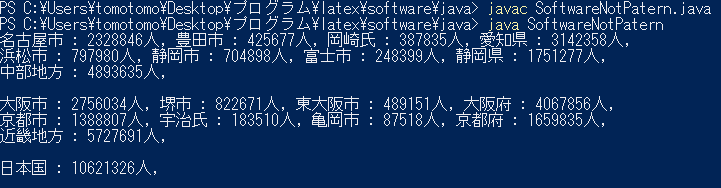
\includegraphics[width=100mm]{kekka.png}
	\end{center}
	\caption{実行したコマンドと動作確認用のデバッグ出力}
	\label{fig:kekka}
\end{figure}

\subsection{作成したプログラム}

\lstinputlisting[caption= パターン未適用 City.java]{./java/City.java}
\lstinputlisting[caption= パターン未適用 Prefecture.java]{./java/Prefecture.java}
\lstinputlisting[caption= パターン未適用 Region.java]{./java/Region.java}
\lstinputlisting[caption= パターン未適用 Country.java]{./java/Country.java}
\lstinputlisting[caption= パターン未適用 SoftwareNotPatern.java]{./java/SoftwareNotPatern.java}

\section{考察}
上記コードの\verb|List<●●> □□ = new ArrayList<>();|となっている部分において、
\verb|<>|の部分がふたつ存在する。この両方を消したものが\ Generics\ 未使用のコードとなる。その場合に、
\ javac\ -Xlink:unChecked\ SoftwareNotPatern.java\ というコマンドを実行してコンパイルしていた。
しかし、\ Generics\ を使用すると、コンパイルコマンドが\ javac\ SoftwareNotPatern.java\  
という形式に短縮されている。これは、型の警告を無視するようなオプションであると考えられる。また、動作としては
そこまで変化しているように感じられなかった。リーフから根に至るように横探索で数字を加算し、
高さを上げていくのである。例えば、中間ノードとして愛知県や静岡県があれば、それらの人口を計算するためには
それぞれの県に属する市の人口を全て加算して、やっとのことでそれらの県の人口が判明する。そのため、
下位のノードのすべての人口の和が計算できるまで、その中間ノードの上に上がることはできない。

\section{感想}
変更せよとのことだったので、変更したコードを貼りました。

\end{document}
